\documentclass[10pt,twocolumn]{IEEEtran11}
\usepackage{listings}
\lstset{
	frame = single, 
	language=C++,
	basicstyle=\tiny}
\usepackage{times}
\usepackage{epsfig}
\usepackage[T1]{fontenc}
\usepackage{graphicx}
\usepackage{subfigure}
\usepackage{tabu}
\def\BibTeX{{\rm B\kern-.05em{\sc i\kern-.025em b}\kern-.08em
    T\kern-.1667em\lower.7ex\hbox{E}\kern-.125emX}}

\oddsidemargin -15pt
\evensidemargin -15pt
\leftmargin 0 pt
\topmargin -30pt
\textwidth = 6.9 in
\textheight = 9.0 in

\newcommand{\itembase}{\setlength{\itemsep}{0pt}}
\newcommand{\eg}{{\it e.g., }}
\newcommand{\ie}{{\it i.e., }}
\graphicspath{{FIG/}}

\begin{document}

\bibliographystyle{IEEE}

\title{\Large \bf A Comparison of Distributed Data Processing Systems}
\author{
Vincent M Chen\\
Information and Computer science Department\\
University of Oregon\\
{\em applekey@cs.uoregon.edu}
}
\maketitle

\section{Introduction}
The explosion of data in the past decade has lead to many questions in finding the most efficient method in order to analyze the data being generated. Best put by Google's CEO, Eric Schmidt, "There were 5 exabytes of information created by the entire world between the dawn of civilization and 2003. Now that same amount is created every two days.", more precisely, in 2003, 6.8 exabytes were being created every 2 days,\cite{gantz2010digital}.  With such a large volume of throughput, trivial tasks such as locating a users' account or finding all users within the same group can't be found in meaningful time with a single computers nor using sequential algorithms.
\par
In order to solve this problem, a very important insight is to notice that a large majority of the data being created is independent from each other, ex. different users on an on-line shopping platform where every shopper has their own independent profile, shopping cart and payment information.  Independence within the data means that parallel computation can be used, where instead of a single computer processing data sequentially, the job is divided into many sub tasks and processed in parallel.  This allows the computation of a large data set to be divided among the processing power of multiple computers.
\par
These parallel computation systems have existed since the 1980's, the most common of which are database systems. In the time since, many database systems have evolved into both parallel and distributed varieties.  As well, alternative computation frameworks introduced recently such as map reduce or Apache Spark have taken a  similarly approach to that used by databases, parallel computation.  The goal of this survey paper is to firstly introduce these different data query systems and their variants.  Secondly, discuss the common approaches all of them use to speed up computation and finally highlight unique aspects of each system.

\section{Basic Description of Functionality}

A data processing solution should satisfy the following functionality:
\begin{enumerate}	
\setlength\itemsep{1em}
	\item Guarantee high degree of fault tolerance.
	\item Compute a user defined query in a reasonable time.
\end{enumerate}

\subsection{Fault Tolerance}
Fault tolerance is the most important guarantee that a computation framework provides.  Without consistency, the data being returned from the query cannot be used for any meaningful analysis. Fault tolerance means recovery from failure from multiple sources
\  \\
\begin{enumerate}
	\setlength\itemsep{1em}
	\item Network fault, communication between compute nodes is unreliable and data is lost in between
	\item System fault, OS failure
	\item Hardware fault, compute computer hard disk fails
	\item User fault, user query has code that leaves query engine in a bad state
\end{enumerate}
\  \\
In order for user defined queries to complete in a reasonable time, two levels of parallelization can be applied.

\subsection{Parallel Computation}
The framework can process independent queries in parallel.  For example, searching for all students who owe more than 10,000 dollars in student loans
can be queried in parallel, each student can be treated independently.

\subsection{Distributed Computation}
The framework is able to distribute the data set across multiple compute machines.  Each machine might contain independent data, for example, one machine contains all students with first names starting A to J and another from K to Z.  Another case is multiple machines hold data that is related to one another.  For example in figure \ref{fig:distDataDependency}, machine A might hold all student's GPA and Awards and another machine holds the student's student loan amount.
If the query were to find all students that had more than 10,000 in student loans but also a 4.0 GPA in order to give them a financial award, then each query per student would need to look at the data in both compute machines.

\begin{figure}[h]
\centering
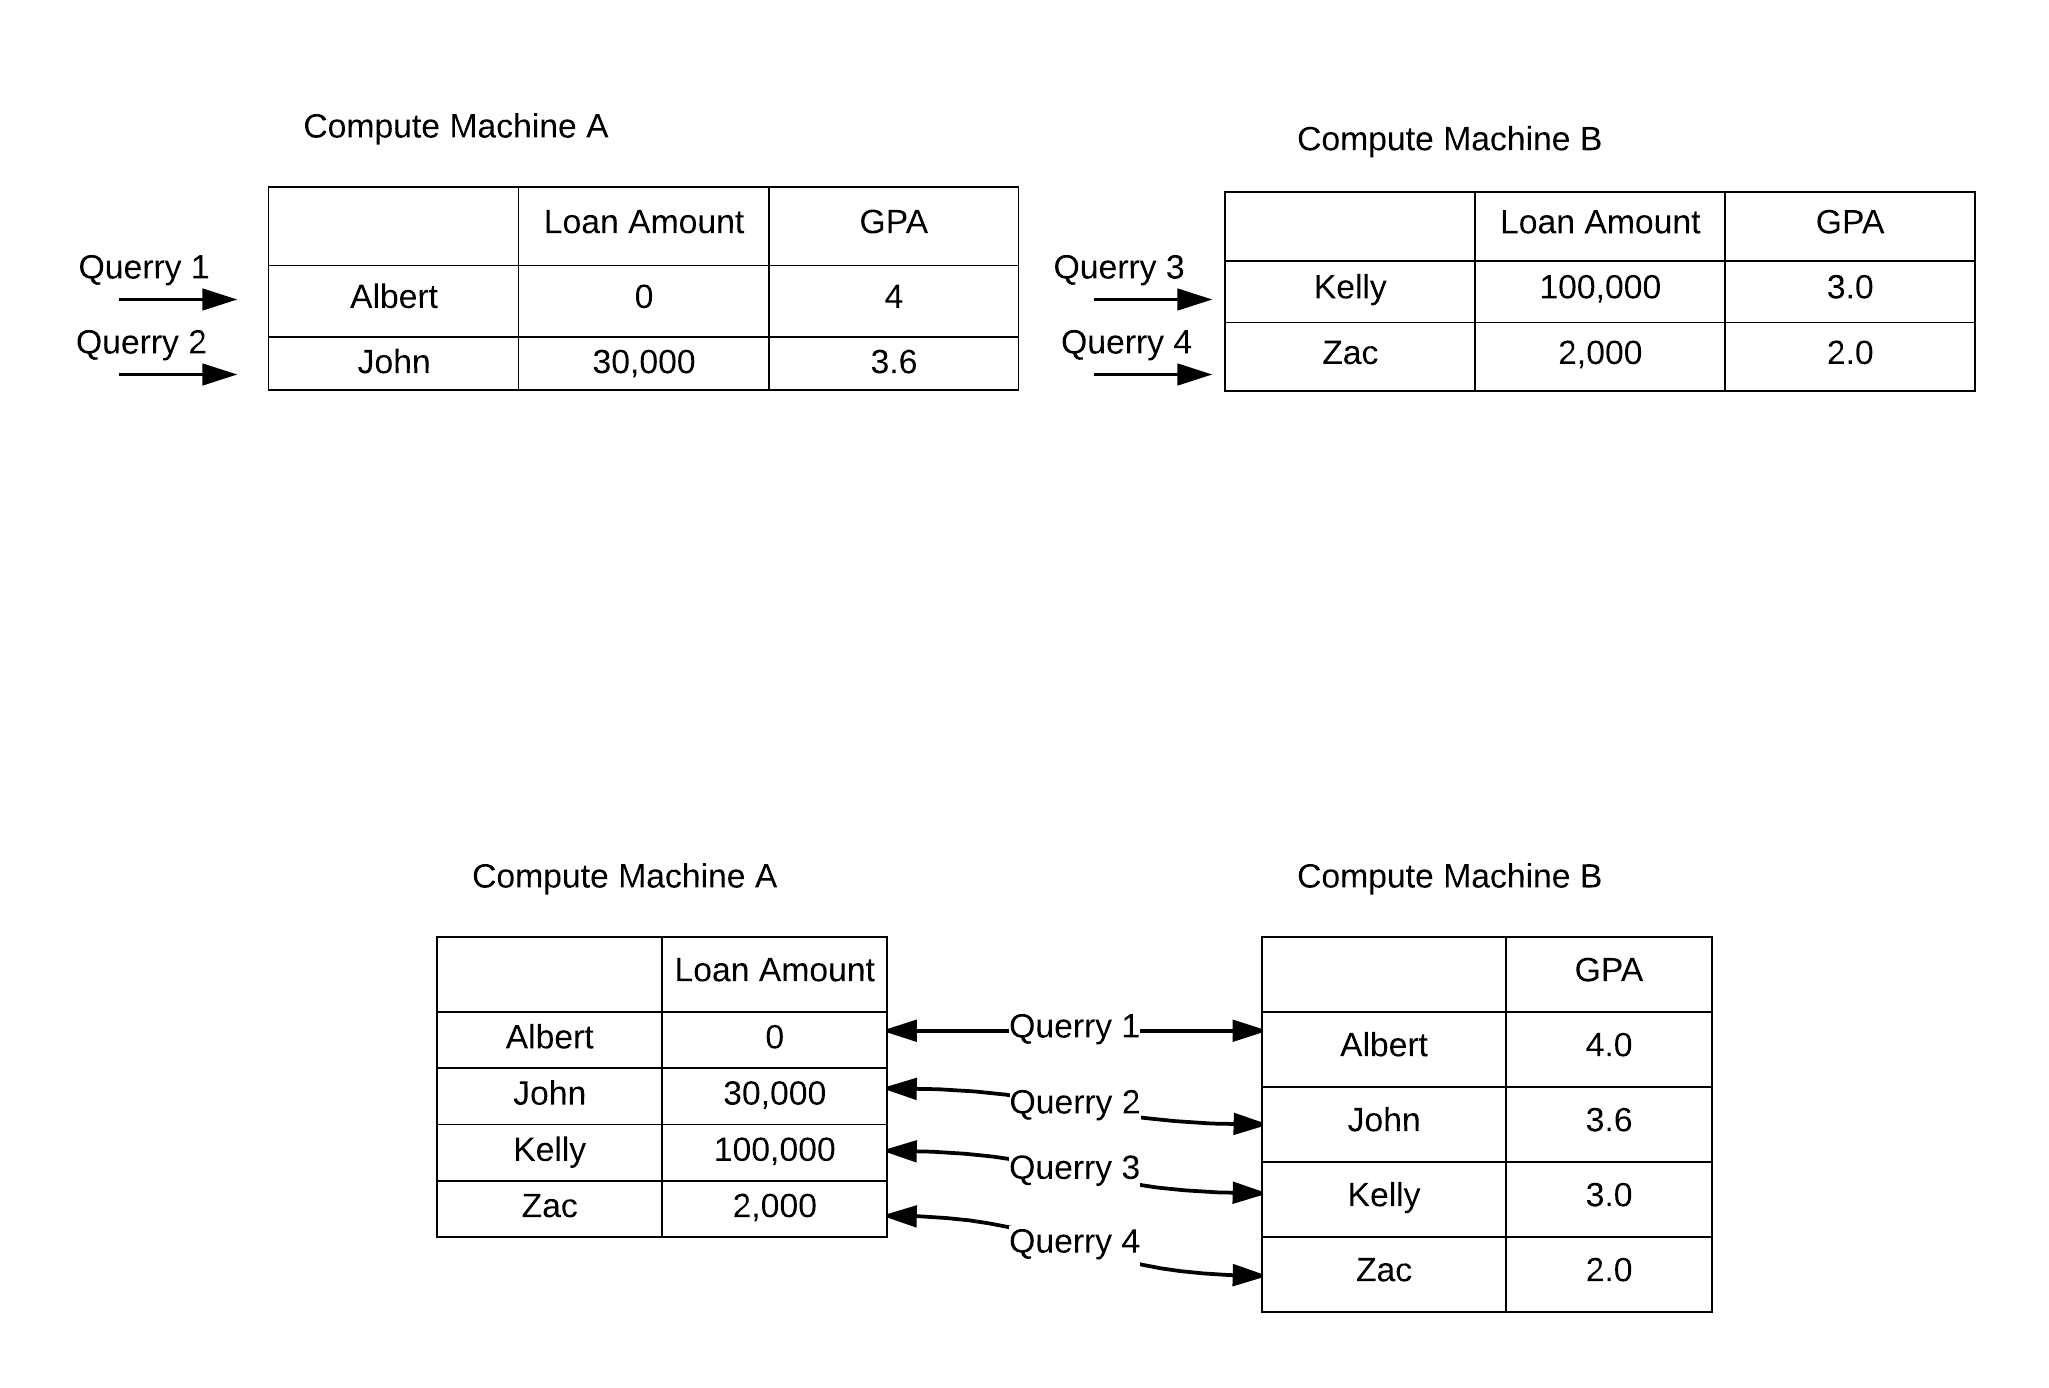
\includegraphics[scale=0.12]{images/parallelComputation.png}
\caption{Distributed Data Dependency}
\label{fig:distDataDependency}
\end{figure}

\section{Databases Management Systems}

Databases management systems are  frameworks that are designed to store data in tabular tables with a set schema.  DBMS systems use relational queries to perform CRUD 
(Create, read, update and delete)operations on the stored data.  

%%\fix{write more here}

\subsection{Parallel DBMS}

Relational queries are ideal suited to run parallel since they
each operation declares independent operations on independent data sets \cite{dewitt1992parallel}.  By partitioning the data among multiple processors, a single query can be carried out in parallel and the result merged into a final step.  In figure \ref{fig:disDBMS}, an independent scan (ex, look for key word) is applied and the results are sorted (binned by first letter) and then the result of each independent operation is merged into the final result.

\begin{figure}[h]
\centering
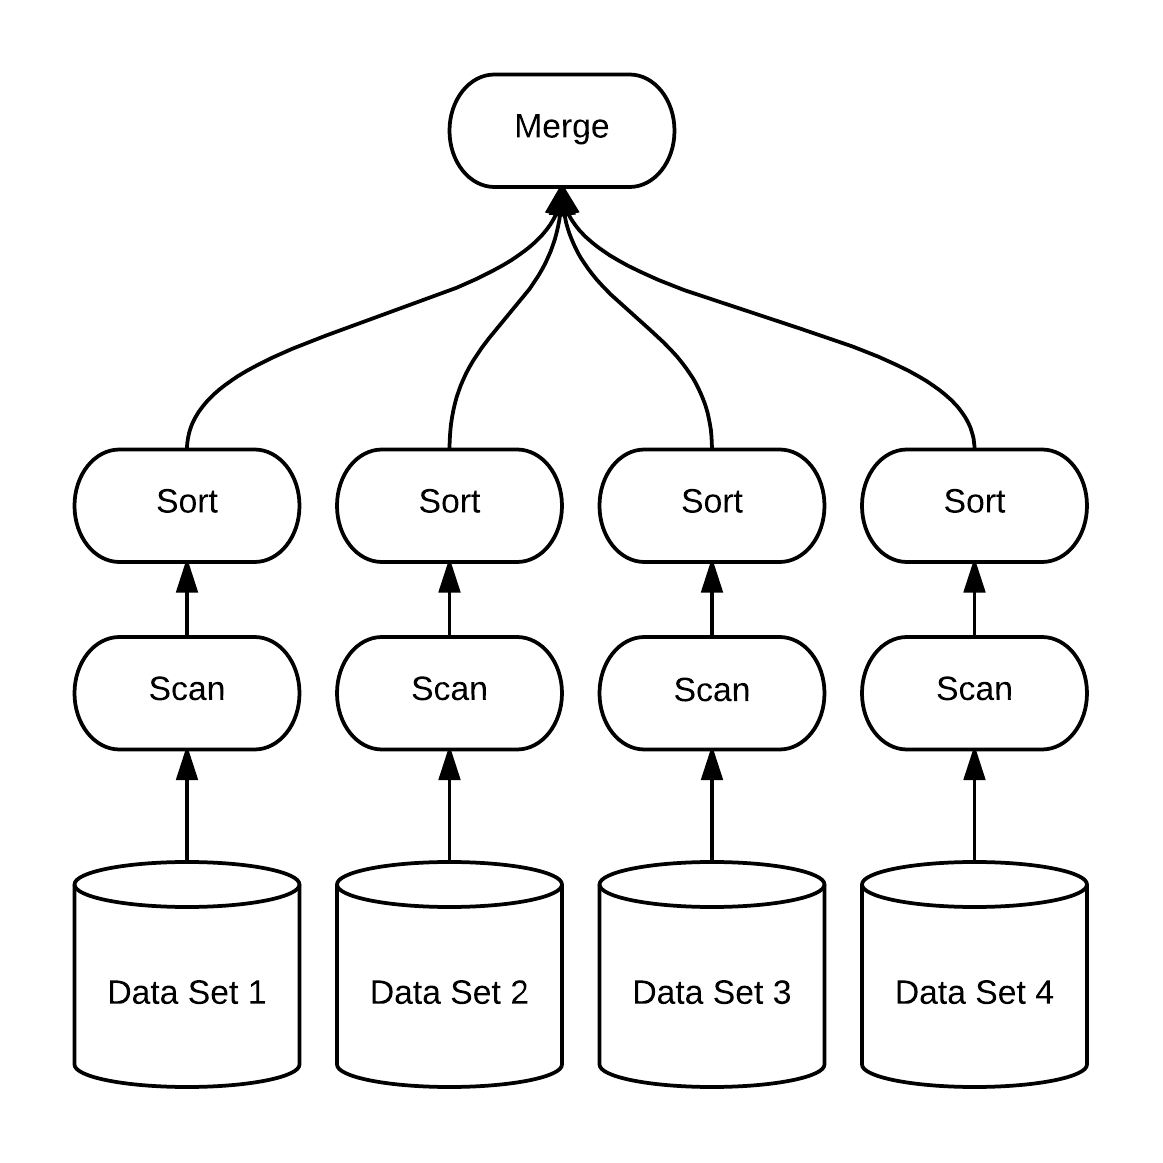
\includegraphics[scale=0.12]{images/parDBMS.png}
\caption{Distributed Data Dependency}
\label{fig:disDBMS}
\end{figure}

\subsection{Distributed DBMS}

Distributed DBMS systems require an additional layer of abstraction on top of Parallel DBMS.  Where as in parallel DBMS systems, all queries are run on the same machine sharing the same memory space.  Distributed DBMS systems need to consider the additional factor of latency when access data that does not reside in the current compute machine.  Additional, distributed DBMS systems need to consider what impact does the memory layout have in preventing easily adding more compute nodes.  

Generally speaking, there are three main types of memory 
architectures for distributed DBMS systems, shared-nothing, shared-memory, shared-disk.
\  \\
\begin{enumerate}
\setlength\itemsep{1em}
\item Shared-Memory: All compute machines share access to a global memory as well as disk storage.  
\item Shared-Disk: Each compute machines have their own memory, but share global disk.
\item Shared Nothing: Each compute machine has their own memory and disk. 
\end{enumerate}

\subsection{Fault Tolerance}
DBMS systems have very mature and well-studied failure mechanisms.  For the purpose of this survey paper, the exact details of each will not be discussed.  DBMS fault tolerance follow the general fault tolerance categories that were described in the general fault tolerance section.  DBMS systems take advantage of the schema and transactions implement restart at different granularity levels.  Through the use of larger compute node level transactions as well as much smaller procedural level transactions, DBMS systems are able to advantage of the work that has already being completed and restart at the most optimal point before the crash.



\section {Map Reduce}

Map Reduce is a general distributed computation framework introduced by Google in 2004 \cite{dean2001mapreduce}.  Map reduce is different from distributed DBMS systems in that much more general computations can be defined, not limited by the query language of a rigid schema as is the case with DBMS systems.  Map Reduce, like DBMS systems have fault tolerance mechanisms but they operate differently than DBMS systems due to the architectural differences. 

\subsection{Mapper and Reducer}
Map reduce operates in two steps, the map step and then the reduce step.  Both steps are independent in that the reduce step will not start until all mappers have completed.
In the map stage, the data is partitioned equally among N mappers.  Input data arrives to the mapper as a list of (key, value) pairs, the mapper applies a user-defined map operation.
The map operation produces an intermediate (key, value) pairs which are the results of the map operations, these results are written and saved to the file system.  
\par
The reducer is again a user defined operation that processes the intermediate values from the mapper grouped by key.  The reducer can produce zero or an aggregate of all values
that map to the same key.

Figure \ref{fig:mapReduce} gives an execution diagram.
\begin{figure}[h]
\centering
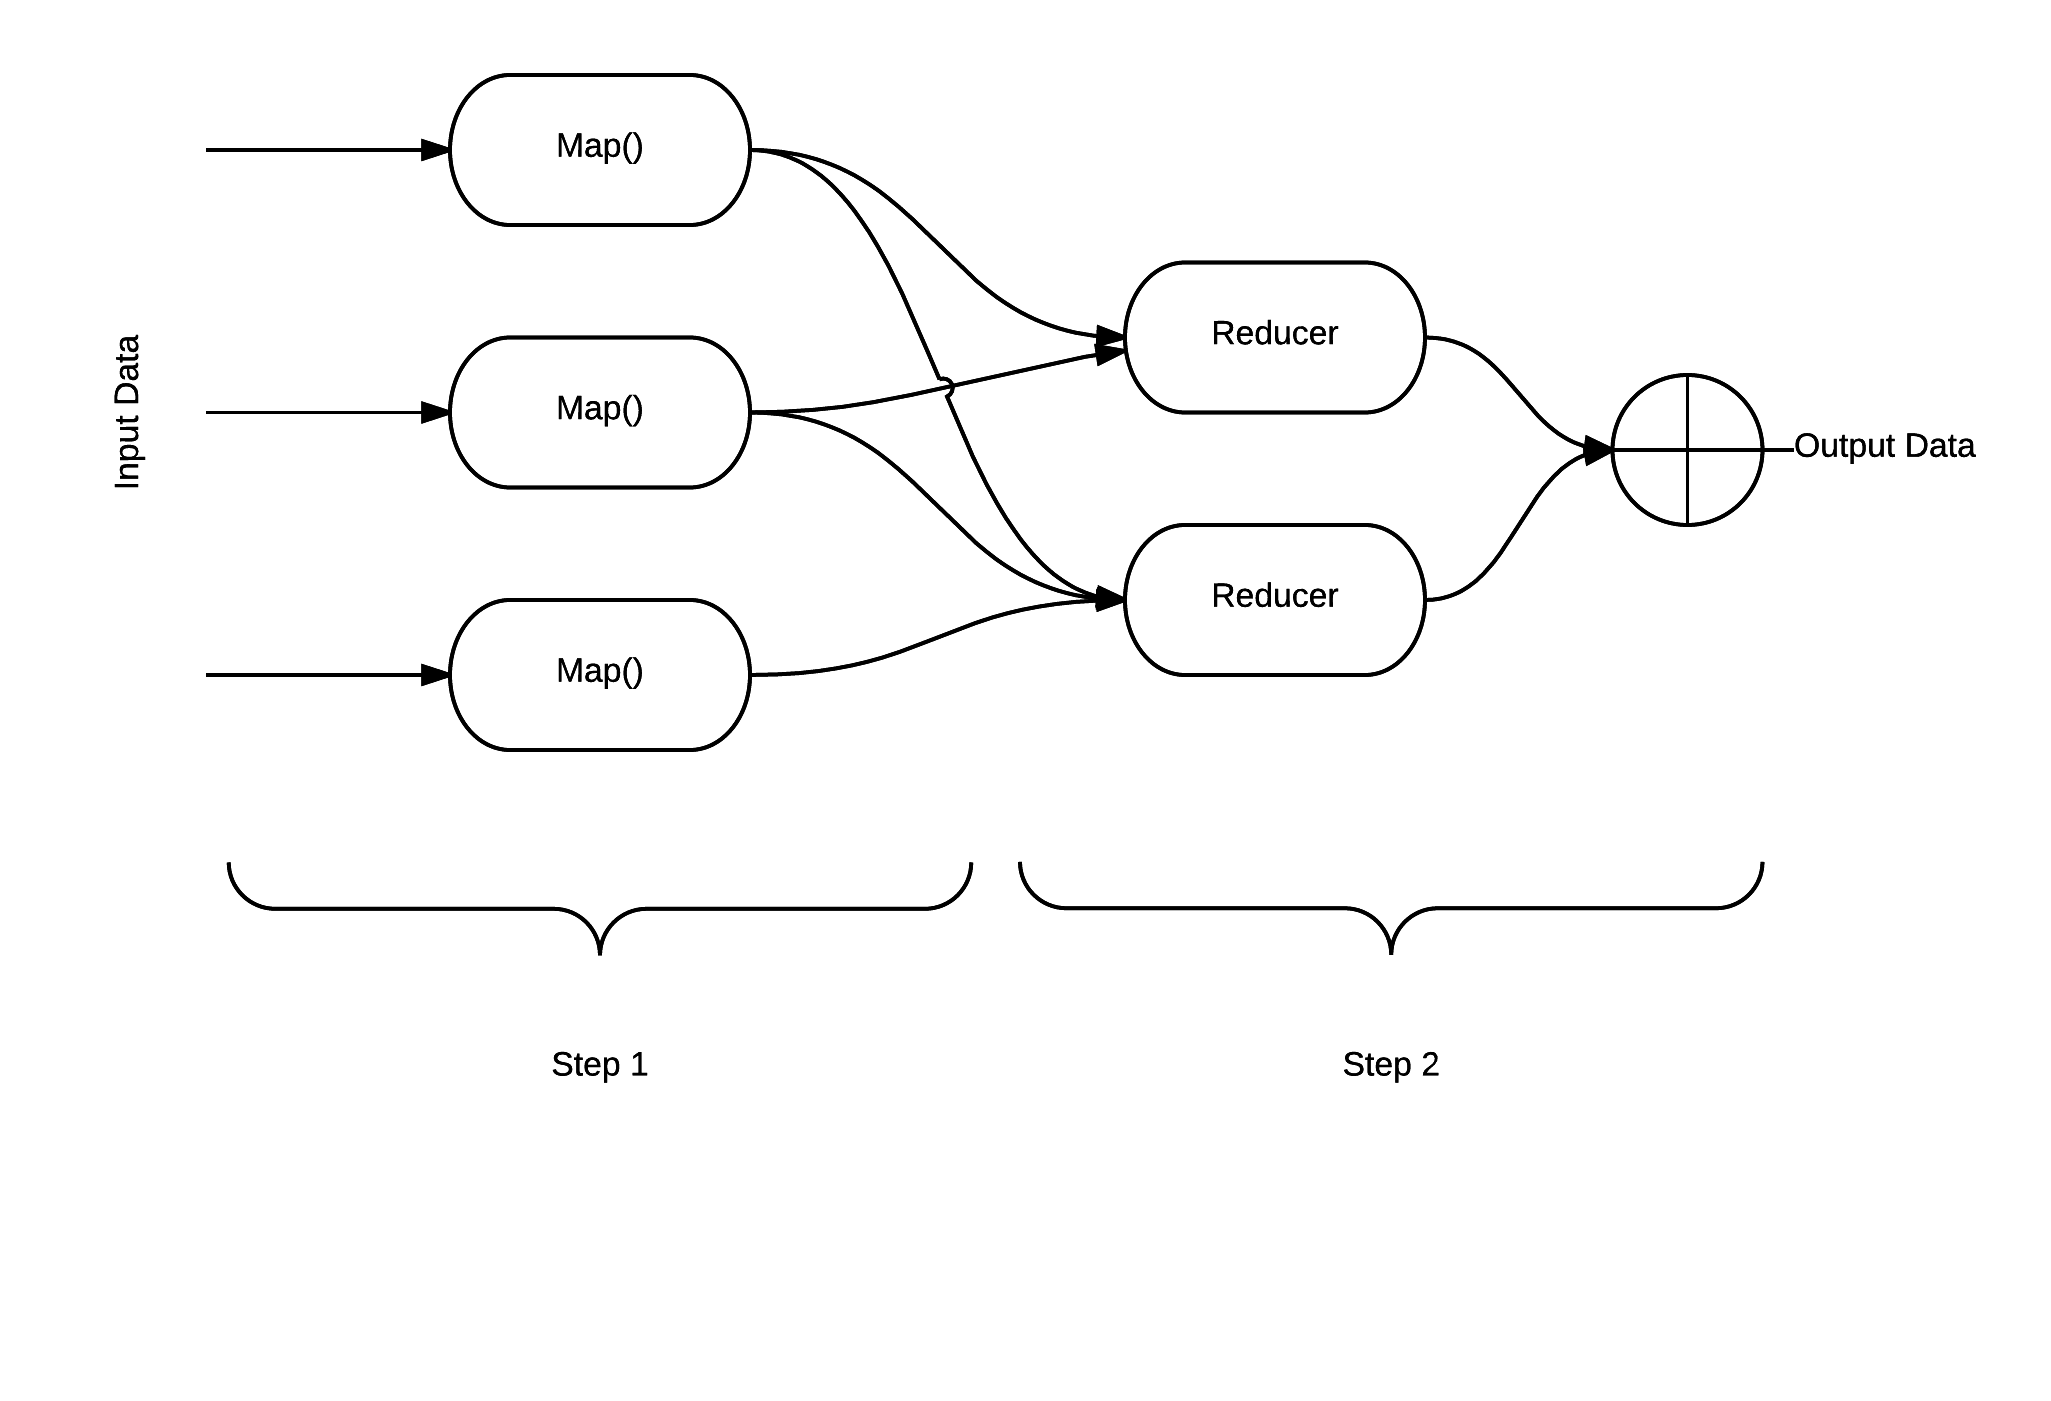
\includegraphics[scale=0.50]{images/mapReduce.png}
\caption{Map Reduce Program Execution}
\label{fig:mapReduce}
\end{figure}

\subsection{Hadoop}
There are two very popular frameworks that implement the map reduce concept, these are the closed source Google Map Reduce and open source version Hadoop Map Reduce.  
This paper will focus on Hadoop instead of Google Map Reduce since the complete details of Google Map Reduce and relatively unknown, however both frameworks function similarly.
\par
Hadoop consist of three layers:
\  \\
\begin{enumerate}
	\setlength\itemsep{1em}
	\item Application layer
	\item Map Reduce layer
	\item HDFS layer
\end{enumerate} 
\  \\
The HDFS layer is Hadoop's storage layer.  The HDFS structures data in blocks that is managed by a master node, when the map reduce runs, the master node will assign each individual mapper data chunks as broken down by the HDFS.  More importantly, the HDFS layer has the is one major component Hadoop Map Reduce's mechanism for
fault tolerance.  The application layer sits on top of the map reduce layer.  The application layer consists of several additions to the standard map reduce framework, these include high level languages, database adaptations.  These application layer additions will be discussed later on in this survey paper.


\subsection{Parallel and Distributed Computation}

The main advantage of the map reduce concept is that there are no dependency between mappers or mappers.  Map reduce therefore is extremely scalable, adding additional nodes either through adding additional cores or compute nodes is a relatively simple task.  This design is very similar to that of the share nothing architecture found in parallel DBMS systems.

\subsection{Fault Tolerance}

Hadoop's fault tolerance mechanism is extremely basics, it achieves fault tolerance through replication.  When a map reduce job is invoked, the input data is triple replicated on the HDFS.  When the mapper or reducer has completed, again the intermediate/final result is triple duplicated.  When the master node, which is responsible for keeping track fo map/reduce jobs notices that a node has failed, the master node will reschedule the map/reduce job with the input/intermediate data.


\section{DBMS vs Map Reduce}
Map reduce and distributed DBMS systems are very similar in that both are parallel data processing frameworks, both support roughly the same feature sets, performance, fault tolerance, user-combustibility.  However, map reduce is far more flexible,  where  as DBMS require data to be organized into schema map reduce can be applied to any variety of data set.  This flexibility is not without its trade-offs though, in general is found to be ~15 - 20 percent slower than that of map reduce in a variety of general tasks \cite{pavlo2009comparison}.  This section will cover the differences between the two and present a performance study between the two.

\subsection{Map Reduce Advantages}

\begin {enumerate}
	\setlength\itemsep{1em}
	\item 
	
	\textbf{Simplicity in Framework}
	
	Programming map reduce is easier to use than query languages such as SQL for two reasons.  Firstly, there are no complex language constructs as is the case with SQL, and secondly, the programmer does not need to understand a table's schema and data layout.
	\item 
	
	\textbf{Flexibility}
	
	The lack of schema's allow data to be organized in any fashion.  The programmer does not need to massage the input data into a rigid format.
	
	\item 
	
	\textbf{Storage Agnostic}
	
	Since there are no set schema's, data can easily be moved from one storage framework (representation) to another.  There is very little needed to re-run the same map/reduce job.  
	For DBMS systems, there would have to be a translation job between two different storage frameworks to ensure that the integrity of the data is kept constant.
	
\end {enumerate}

\subsection{Map Reduce Disadvantages}


\begin {enumerate}
\setlength\itemsep{1em}
\item 

\textbf{Lack of High Level Language}

While map reduce is extremely to program due to the simplistic nature of the logical map and reduce function, the lack of a high level language means that there is very little in terms of portability when multiple map reduce stages are chained together.   Take for example, a very common query in SQL, select * from table where column 1 > value 1 and column 2 > value 2.  In map reduce, there would be two stages, the first stage
would filter by column 1 and the second column 2.  The programmer would need to know to pass data from column 1 in first, then pass in data from column 2.  The programmer cannot pass in an entire row with multiple columns because map reduce only supports single (key,value ) pairs.
In this regards, map reduce has often being compared with assembly programming, it is difficult to re-use a preexisting map reduce stage without knowing entirely the execution flow for it.  
\item 

\textbf{Rigid Data Flow}

Map reduce runs in two discrete steps, the reduce step does not start until all the mapper steps have completed.  Since map reduce is a distributed system running on any kind of network, the possibility that there is a single straggler node is entirely not out of the ordinary.  In this situation, all compute nodes would have to wait on the straggler node.  DBMS systems do not have this constraint, using the Schema and query logic, the scheduler will schedule as many local reduces as possible from free compute nodes, this results faster execution times \cite{yang2007map}.

\item 

\textbf{Lack of Schema or Indexes}

One of map reduce's biggest advantages, flexibility is also one of its largest disadvantages.  While not having a schema means that map reduce jobs have very fast initiation times,  on the other searching operations  are considerable slower.  A lack of schema also means that between multiple map reduce stages, data has to be parsed again and again.  In addition, the lack of a schema means that compile time optimizations cannot be made, only runtime optimizations as well, reductions in logic between multiple map reduce stages.

\end {enumerate}


\subsection{Difference in Programming Model}
%% -> I think this section should be moved into the high level language section
Map reduce and DBMS represent an old discussion on two different views in methods to access data \cite{pavlo2009comparison}.  These are:
\  \\
\begin{enumerate}
	\setlength\itemsep{1em}
	\item Relational view, state what you want rather than presenting an algorithm; this represents map reduce.
	\item Codasyl, an algorithm for data access; this represents query languages such as SQL.
\end{enumerate} 
\  \\
At the time, it was concluded that relational are easier to understand and modify with Codasyl being criticized for being "too assembly similar to assembly".  

\section{Map Reduce versus DBMS Performance}

Hadoop Map Reduce and Parallel DBMS systems compared in performance for three category of tasks on a 100 node cluster.  The execution times between the two are presented in table \ref{table:hadoopVsDBMS}.  

\subsection{System Configurations}
Both map reduce and DBMS systems were deployed on a 100 node cluster.  Each node has a single 2.40 GHz Intel Core 2 Duo with 4GB of ram and two 250GB SATA-I hard disks.  All 100 nodes were connected using two gigabyte 128 Gbps Ethernet switch with 50 nodes per switch.

\subsection{Grep Task}

The first task was the grep task as was presented in the original Google Map Reduce paper.  This task involved searching for a specific keyword that occurred once every 1000 (key, value) pairs.   The total data set consisted of 1 TB split amount 100 nodes.  Per node, 10 GB of records consisting of 100B records was partitioned to assigned map tasks.  This test was designed to measure pure IO throughput of the two systems.  This grep task is designed such that both Hadoop Map Reduce and DBMS-x are not able to take advantage of indexes.  In addition, there is no reduce step in this experiment since if the specific keyword is found, it is outputted as the result.
\par
One would expect Hadoop to perform well in comparison to DBMS-x since Hadoop has a much simpler initialization mechanism, simply load data via (key, value) pairs.  However, referring to table \ref{table:hadoopVsDBMS}, Hadoop was 1.5 slower.  This slow down can be attributed to the need for repetitive record record parsing.  Since Hadoop does not have any special storage formats, such as DBMS data indexing and messaging, it is up to the use's code to  read in and write out data in the appropriate format.  In Hadoop's native language Java, (key, value) pairs are stored as immutable strings.  This means anytime any modification on any (key,value) pairs are done, the original string is deleted and re-created in memory.
\par
Secondly, DBMS systems are well matured products with highly efficient data compression algorithms.  In the study, it was found that enabling compression on DBMS systems enabled performance by a factor of two to four \ref{table:hadoopVsDBMS}.  On the other hand, there has not being a lot of work on Hadoop and data compression, at most a 15 percent performance boost was seen \cite{dean2001mapreduce}.

\subsection{Web Log Task}
The second task is a SQL aggregation, "GROUP BY" clause on a table of user visits in a Web server log.  The data set used is a 2TB data set with a total of 155 million records distributed over 100 nodes, translating to 20 GB of data per node.  Each node runs the group by and records to total ad revenue for each IP address.  Similar to the previous Grep experiment, all records must be scanned and there no advantage is gained from indexing.  This experiment involves a reduce step in order to collect all visits from different IP addresses.
\par
Again, Hadoop is considerably slower than DBMS-x in performance.  The addition of a reduce step, where (key,value) immutable string pairs have to be serialized and de serialized may be the reason why this task has worse performance than the Grep task.

\subsection {Join Task}
The final task is a situation where map reduce model is inadequate in handling. The final task consist of a complex join operation over two tables which require both an aggregation and then filtering.   The data set utilizes the use visits from the previous join task joined with another 100 GB table of PageRank values that consist of 18 million URL's.  The first part consists of the system locating the IP address that generates the most revenue within a set range in the user visits data set.  The intermediate result records are then joined with the PageRank table and used to calculate the average Page Rank of all the pages visited during this interval.   Referring to table \ref{table:hadoopVsDBMS}, Hadoop is considerably, 36.3x slower than DBMS systems.  In the next paragraph, we will given some insight as to why the map reduce model fails so far when it comes to joins.

\begin{table}[h!]
	\centering
\begin{tabu} to 0.4\textwidth { | X[l] | X[c] | X[r] | X[l] |}
	\hline
    & Hadoop & DBMS-x & Hadoop/DBMS-x\\ 
	\hline
	Grep  & 284s  & 194s  & 1.5x  \\
	\hline
	Web Log  & 1,146s  & 740s& 1.6x  \\
	\hline
	Join  & 1,1158s  & 32s& 36.3x  \\
	\hline
\end{tabu}
\caption{Hadoop vs DBMS-x performance}
\label{table:hadoopVsDBMS}
\end{table}

\section{Joins in DBMS vs Map Reduce}

Take an example data set consisting of two tables, Employees and Department
\begin{table}[h!]
	\centering
	\begin{tabu} to 0.4\textwidth { | X[l] | X[c] | X[r]  |}
		\hline
		Name & Age & Dept Id\\ 
		\hline
		Alex  & 26  & 2  \\
		\hline
		Ben & 24  & 2  \\
		\hline
		Sarah  & 34  &5  \\
		\hline
	\end{tabu}
	\caption{Employees Table}
	\label{table:}
\end{table}

\begin{table}[h!]
	\centering
	\begin{tabu} to 0.4\textwidth { | X[l] | X[c] |}
		\hline
		 Department Id & Name\\ 
		\hline
		5  & Marketing   \\
		\hline
		2  & Engineering    \\
		\hline
		3& Sales  \\
		\hline
	\end{tabu}
	\caption{Hadoop vs DBMS-x performance}
	\label{table:hadoopVsDBMS}
\end{table}

Suppose the following Join was carried out, " Select * from Employees join Department on Employees.DepartmentId = Department.DepartmentId".
When this query is run on a DBMS system, the system has two options, in most situations' it will use the data's indexes to its advantage and carry out a hash join which is $O(1)$ time or at worst carry out a index join,$ O(log N) $time.  Also, all data representations are internally maintained in the database and no extraneous conversions are carried out.
\par
Having this query carried out through Map Reduce runs through a similar execution model, first a filter then an aggregate.  However, since the data have no indexes, hashing and divide and conquer techniques cannot be applied.  Every operation between the two tables is an $O(n^2)$ operation.  As well, there are extraneous serialization/de-serialization steps in between the map and filter steps.  The following section gives an example flow diagram as well as mapper and reduce pseudo code to demonstrate the join \cite{afrati2010optimizing}.

\subsection{Map Reduce Join}

Joins in map reduce are run in $O(n^2)$ time due to lack of help from indexes or any table schema.  In the first stage, the mapper maps both tables using the join column as the key, this produces the intermediate results as shown in figure \ref{fig:mrJoin}, stage 1.  In stage 2, the mapper's local aggregation pairs all values per key, now both employees and department records share the same key. In stage 3, the reducer  runs a double for loop, looping through each employee record in the outer loop and then each department record in the inner loop, if the value's tag is not the same tag as the outer loop's tag, this means that these two values need to be joined.  The reducer's code for stage is include in code listing \ref{joinCode}, take note of line 5 as well line 6, where the tag comparison for tags as well join of values are run, these are expensive Java string operations. 


\begin{figure}[h]
	\centering
	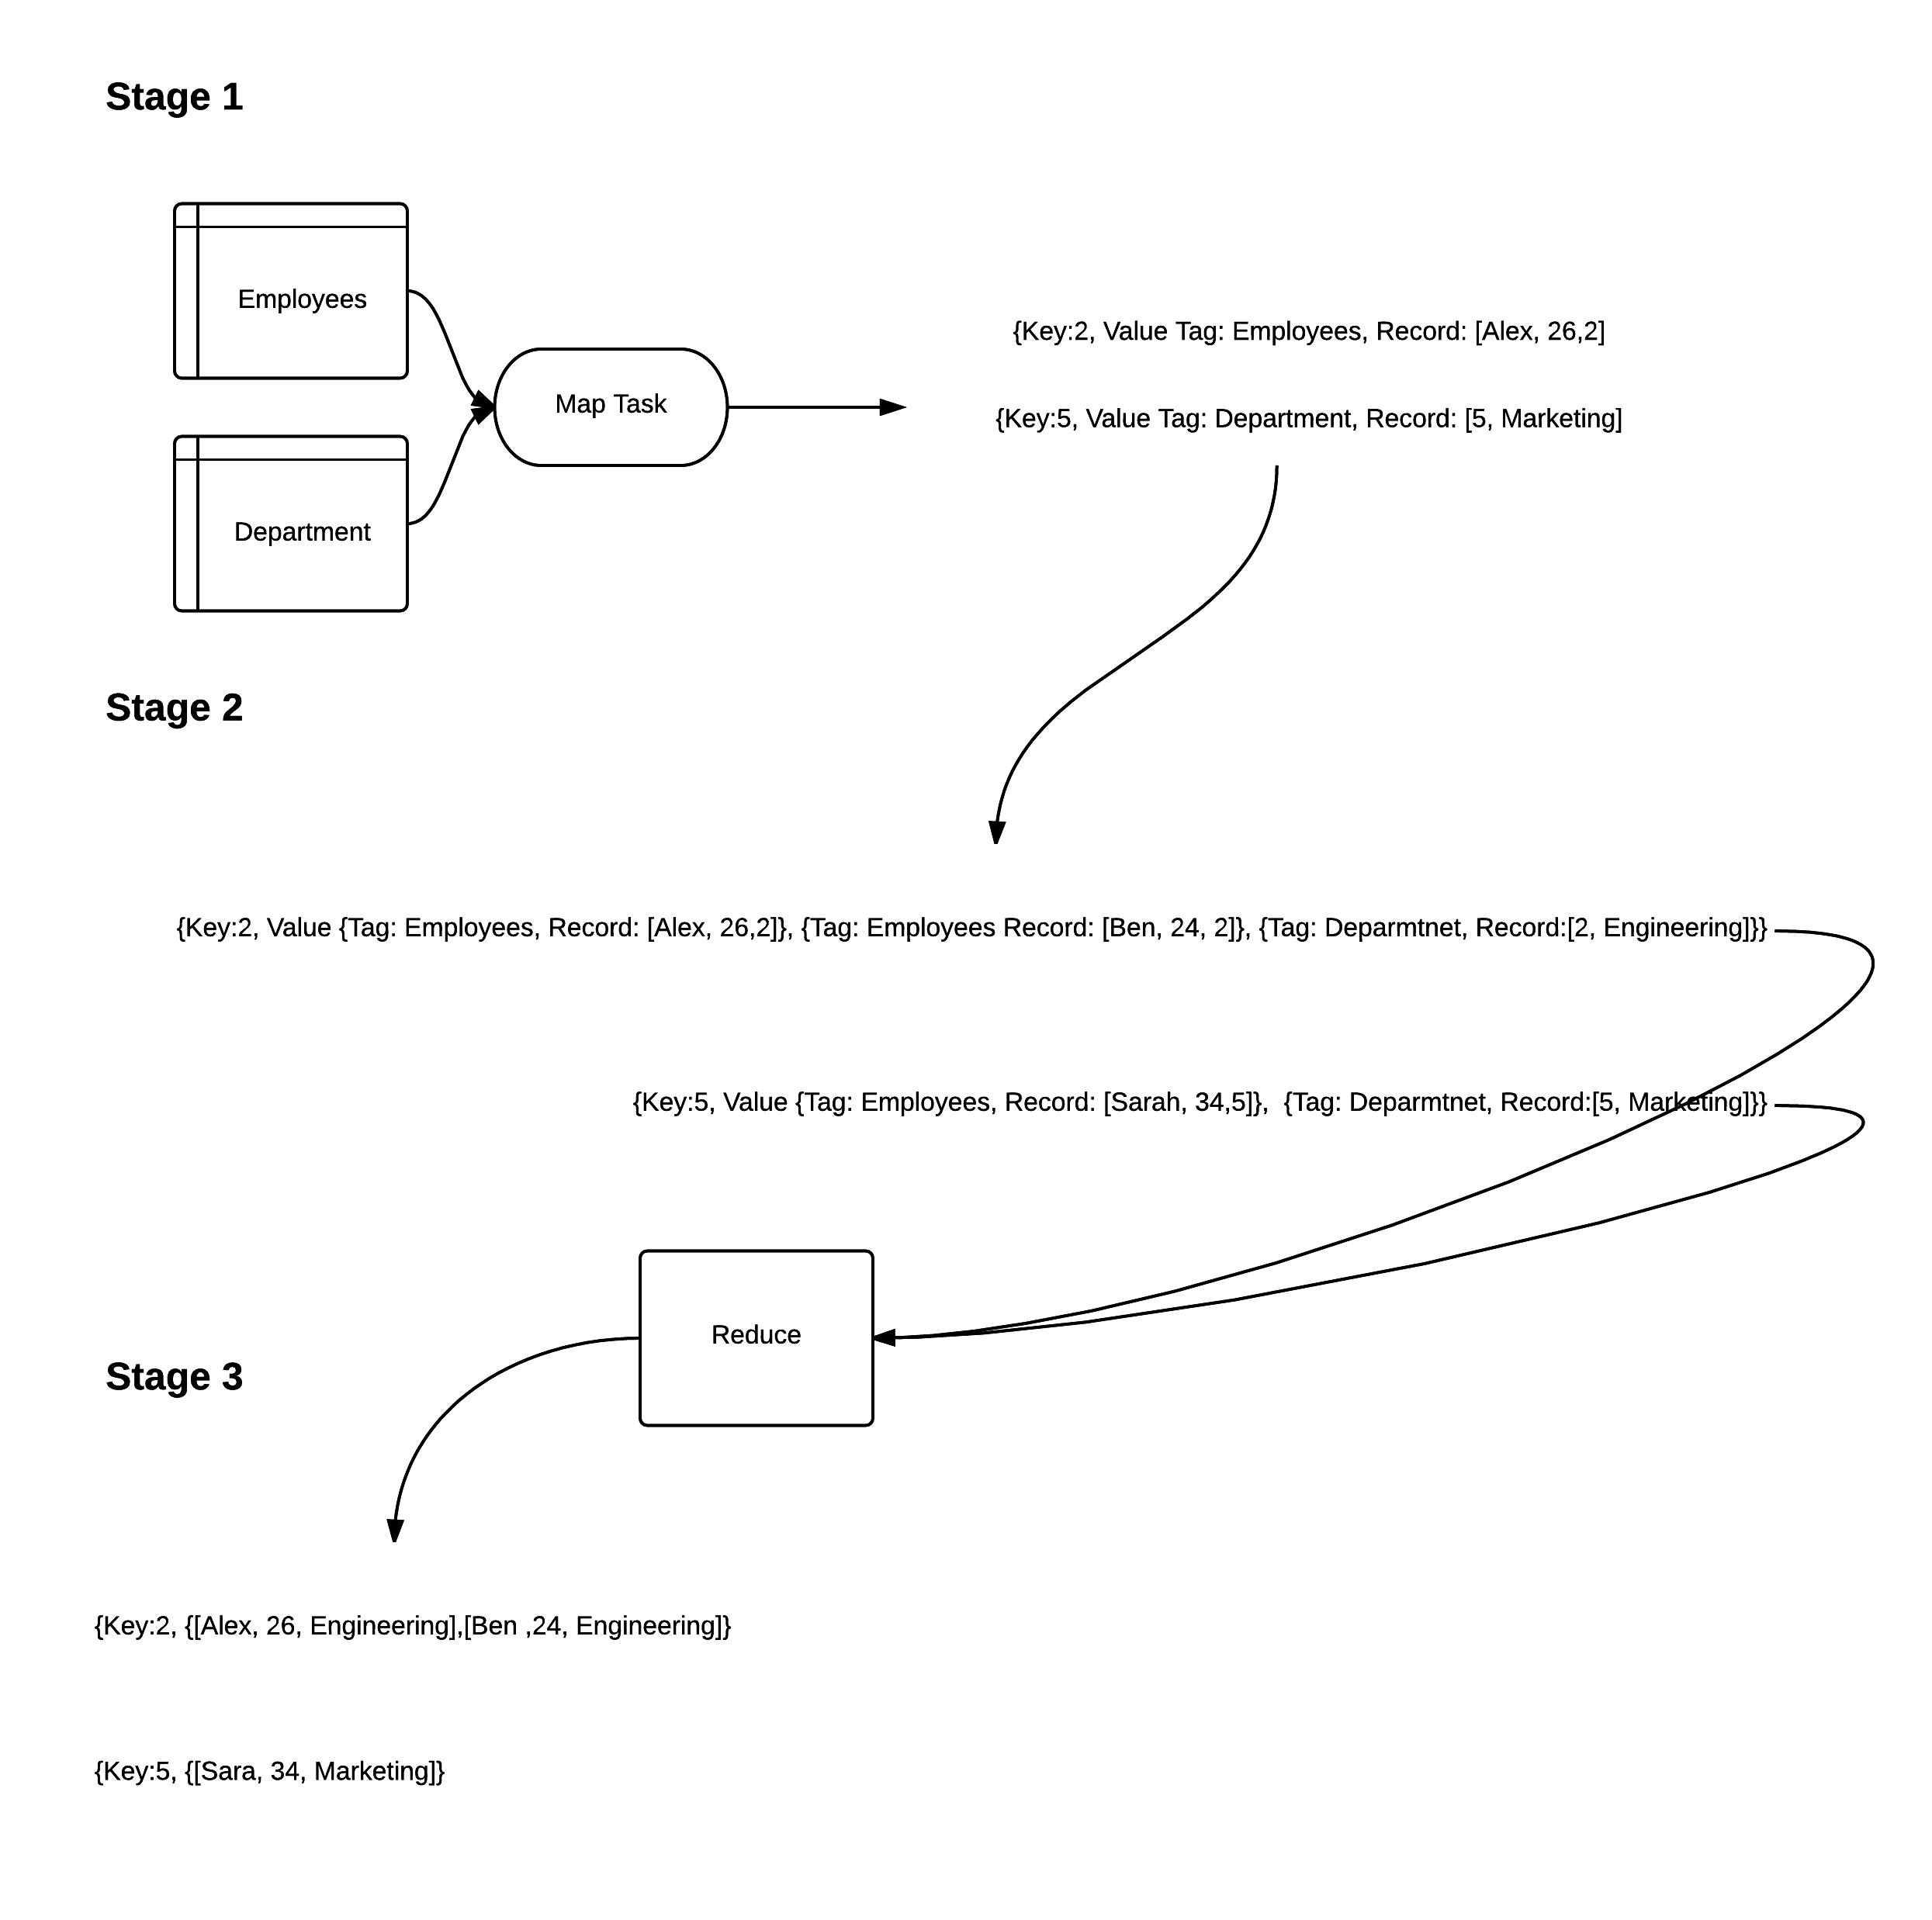
\includegraphics[scale=0.5]{images/mapReduceJoin.png}
	\caption{Join stages in map reduce}
	\label{fig:mrJoin}
\end{figure}

\begin{lstlisting} [caption=Reducer code,label=joinCode]
1. reduce (K dept_id, list<tagged_rec> tagged_recs)  {
2.  for (tagged_rec : tagged_recs) {
3.    for (tagged_rec1 : taagged_recs) {
4.	  if (tagged_rec.tag != tagged_rec1.tag) {
5.	    joined_rec = join(tagged_rec, tagged_rec1)
6.  }
7.  emit (tagged_rec.rec.Dept_Id, joined_rec)
8.  }
9. }
\end{lstlisting}



\section{fdsafdsafsad}

in \ref{joinCode}




























\bibliography{citations}


\end{document}
